\documentclass[oneside, 12 pt, leqno]{memoir}
\usepackage{standalone}
\usepackage[dvips,text={6.2in,8.5in},left=0.9truein,top=1.5truein]{geometry}
\usepackage{amsmath, amssymb, amsthm, amsfonts}
\usepackage{graphicx}
\usepackage{titlesec}
\usepackage{multirow}
\usepackage{wrapfig}
\usepackage{microtype}
\usepackage{indentfirst}
\usepackage[utf8]{inputenc}
\usepackage{exscale}
\usepackage{mlmodern}
\usepackage[OT1]{fontenc}
\usepackage[bottomfloats]{footmisc}
\parindent=2.27em
\parskip=0pt
\nonfrenchspacing
\renewcommand{\baselinestretch}{1.15}
\DeclareMathSizes{12}{12}{8}{6}
\everymath{\displaystyle}
\allowdisplaybreaks
\raggedbottom
\titleformat{\section}
  {\normalfont\centering}{\thesection.}{1em}{}
\titleformat{\subsection}
  {\normalfont\normalsize\centering}{\thesection.}{1em}{}
\titleformat{\subsubsection}
  {\normalfont\normalsize\centering}{\thesection.}{1em}{}
\spaceskip=0.67em plus 0.33em minus 0.33em
\thickmuskip=4mu plus 4mu
\medmuskip=3mu plus 1.5mu minus 3mu
\AtBeginDocument{%
  \mathchardef\stdcomma=\mathcode`,
  \mathcode`,="8000
}
\begingroup\lccode`~=`, \lowercase{\endgroup\def~}{\stdcomma\mspace{\medmuskip}}
\let\oldfrac\frac
\def\frac#1#2{\mathchoice{\text{\scalebox{.83}{${\oldfrac{#1}{#2}}$}}}{\text{\scalebox{.83}{${\displaystyle\oldfrac{#1}{#2}}$}}}{\genfrac{}{}{}{2}{#1}{#2}}{\genfrac{}{}{}{3}{#1}{#2}}}
\begin{document}
\setlength{\abovedisplayskip}{0.33\baselineskip plus .16\baselineskip minus .16\baselineskip}
\setlength{\belowdisplayskip}{0.33\baselineskip plus .16\baselineskip minus .16\baselineskip}

\;\\ [3\baselineskip]
\section*{\begin{Large}II.\end{Large} \\ [\baselineskip]
SOLUTION OF SOME PROBLEMS USING DEFINITE INTEGRALS}
\begin{center}
\rule{2in}{0.1pt}\\ [0.5\baselineskip]
\begin{scriptsize}Magazin for Naturvidenskaberne, Aargang I, Bind, Christiania 1823\par\end{scriptsize}
\rule{2in}{0.1pt}
\end{center}

\subsection*{1.}

It is well known that many problems that otherwise cannot be solved, or at least are very difficult to treat, can be solved using definite integrals. These have been particularly advantageously applied to the solution of several difficult problems in mechanics, for example, to the motion of an elastic surface, problems in the theory of waves, etc. I will provide a new application by solving the following problem.

\begin{wrapfigure}{L}{4.5\baselineskip}
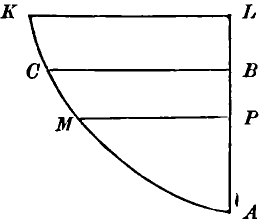
\includegraphics[width=4.5\baselineskip]{Tome_I_Ouevre_II_Fig_1.png} 
\end{wrapfigure} 

Let \(CB\) be a horizontal line, \(A\) a given point, \(AB\) perpendicular to \(BC\), \(AM\) a curve with rectangular coordinates \(AP=x\), \(PM=y\). Let \(AB=a\), \(AM=s\). If we now imagine that a body moves on the arc \(CA\), with initial velocity zero, the time \(T\) it takes to traverse it will depend on the shape of the curve and on \(a\). The task is to determine the curve \(KCA\) such that the time \(T\) is equal to a given function of \(a\), e.g. \(\psi(a)\).

If we denote by \(h\) the velocity of the body at point \(M\), and by \(t\) the time it takes to travel the arc \(CM\), we have as we know
\[h=\sqrt{BP}=\sqrt{a-x}, dt=-\frac{ds}{h},\]
thus
\[dt=-\frac{ds}{\sqrt{a-x}},\]
and by integrating
\[t=-\int \frac{ds}{\sqrt{a-x}}.\]
To obtain \(T\) we must take the integral from \(x=a\) to \(x=0\), thus we have
\[T=\int_{x=0}^{x=a} \frac{ds}{\sqrt{a-x}}.\]
Now since \(T\) is equal to \(\psi a\), the equation becomes
\[\psi a=\int_{x=0}^{x=a} \frac{ds}{\sqrt{a-x}}.\]
Instead of solving this equation, I will show how one can obtain \(s\) from the more general equation
\[\psi a=\int_{x=0}^{x=a} \frac{ds}{(a-x)^n},\]
where \(n\) is assumed to be less than unity, so that the integral does not become infinite between the given limits; \(\psi a\) is an arbitrary function that does not become infinite when \(a\) is zero.

Let us define
\[s=\Sigma \alpha^{(m)} x^m,\]
where \(\Sigma {\alpha}^{(m)} x^m\) has the following value:
\[\Sigma {\alpha}^{(m)} x^m={\alpha}^{\left(m^{\prime}\right)} x^{m^{\prime}}+{\alpha}^{\left(m^{\prime \prime}\right)} x^{m^{\prime  \prime}}+\alpha^{\left(m^{\prime \prime \prime}\right)} x^{m^{\prime \prime \prime}}+\ldots.\]
Differentiating, we obtain
\[d s=\Sigma m \alpha^{(m)} x^{m-1} d x,\]
so
\[\frac{d s}{(a-x)^n}=\frac{\Sigma m \alpha^{(m)} x^{m-1} d x}{(a-x)^n}={\Sigma m} \alpha^{(m)} \frac{x^{m-1} d x}{(a-x)^n}.\]
Integrating, we have
\[\int_{x=0}^{x=a} \frac{d s}{(a-x)^n}=\int_{x=0}^{x=a} \Sigma m \alpha^{(m)} \frac{x^{m-1} d x}{(a-x)^n}.\]
Now
\[\int \Sigma m \alpha^{(m)} \frac{x^{m-1} d x}{(a-x)^n}=\Sigma m \alpha^{(m)} \int \frac{x^{m-1} d x}{(a-x)^n},\] 
so, since \( \int_{x=0}^{x=a} \frac{d s}{(a-x)^n}=\psi a\):
\[\psi a= \Sigma m \alpha^{(m)} \int_0^a \frac{x^{m-1} d x}{(a-x)^n}.\]
The value of the integral
\[\int_0^a \frac{x^{m-1} d x}{(a-x)^n}\]
is easily found as follows: If we let \(x=a t\), we have
\[\begin{gathered}
x^m=a^m t^m, m x^{m-1} d x=m a^m t^{m-1} d t \\
(a-x)^n=(a-a t)^n=a^n(1-t)^n,
\end{gathered}\]
so
\[\frac{m x^{m-1} d x}{(a-x)^n}=\frac{m a^{m-n} t^{m-1} d t}{(1-t)^n},\]
and by integrating
\[m \int_0^a \frac{x^{m-1} d x}{(a-x)^n}=m a^{m-n} \int_0^1 \frac{t^{m-1} d t}{(1-t)^n}.\]
Now we have
\[\int_0^1 \frac{t^{m-1} d t}{(1-t)^n}=\frac{\Gamma(1-n) \Gamma m}{\Gamma(m-n+1)},\]
where \(\Gamma m\) is a function determined by the equations
\[\Gamma(m+1)=m \Gamma m, \Gamma(1)=1.\footnote{The properties of this remarkable function have been extensively developed by Mr. \textit{Legendre} in his work, Exercises in Integral Calculus Vol. I and II.}\]
Substituting this value for the integral \(\int_0^1 \frac{t^{m-1} d t}{(1-t)^n}\), and noting that \(m \Gamma m=\Gamma(m+1)\), we have
\[m \int_0^a \frac{x^{m-1} d x}{(a-x)^n}=\frac{\Gamma(1-n) \Gamma(m+1)}{\Gamma(m-n+1)} a^{m-n}.\]
Substituting this value in the expression for \(\psi a\), we obtain
\[\psi a=\Gamma(1-n) \Sigma \alpha^{(m)} a^{m-n} \frac{\Gamma(m+1)}{\Gamma(m-n+1)}.\]

Letting
\[\psi a=\Sigma \beta^{(k)} a^k,\]
we have
\[\Sigma \beta^{(k)} a^k=\sum \frac{\Gamma(1-n) \Gamma(m+1)}{\Gamma(m-n+1)} \alpha^{(m)} a^{m-n}.\] 
For this equation to hold, we need \(m-n=k\), which implies \(m=n+k\), and
\[\beta^{(k)} = \frac{\Gamma(1-n) \Gamma(m+1)}{\Gamma(m-n+1)} \alpha^{(m)}=\frac{\Gamma(1-n) \Gamma(n+k+1)}{\Gamma(k+1)} \alpha^{(m)},\]
thus
\[\alpha^{(m)}=\frac{\Gamma(k+1)}{\Gamma(1-n) \Gamma(n+k+1)} \beta^{(k)}.\]
Now we have
\[\int_0^1 \frac{t^k d t}{(1-t)^{1-n}}=\frac{\Gamma n. \Gamma(k+1)}{\Gamma(n+k+1)},\]
therefore
\[\alpha^{(m)}=\frac{\beta^{(k)}}{\Gamma n. \Gamma (1-n)} \int_0^1 \frac{t^k d t}{(1-t)^{1-n}}.\]
Multiplying by \(x^m=x^{n+k}\), we obtain
\[\alpha^{(m)} x^m=\frac{x^n}{\Gamma n. \Gamma(1-n)} \int_0^1 \frac{\beta^{(k)}(x t)^k d t}{(1-t)^{1-n}},\]
hence
\[\Sigma \alpha^{(m)} x^m=\frac{x^n}{\Gamma n. \Gamma(1-n)} \int_0^1 \frac{\Sigma \beta^{(k)}(x t)^k d t}{(1-t)^{1-n}}.\]
But we have \(\Sigma {\alpha}^{(m)} x^m=s\), \(\Sigma \beta^{(k)}(x t)^k=\psi(x t)\), thus
\[s=\frac{x^n}{{\Gamma n}. {\Gamma}(1-n)} \int_0^1 \frac{\psi(x t) d t}{(1-t)^{1-n}}.\]
Using the identity \(\Gamma n. \Gamma(1-n)=\frac{\pi}{\sin n \pi}\), we can write
\[s=\frac{\sin n \pi. x^n}{\pi} \int_0^1 \frac{\psi(x t) d t}{(1-t)^{1-n}}.\]

From the above, the following remarkable theorem follows:

If we have
\[\psi a=\int_{x=0}^{x=a} \frac{d s}{(a-x)^n},\]
then we also have
\[s=\frac{\sin n \pi}{\pi} x^n \int_0^1 \frac{\psi(x t) d t}{(1-t)^{1-n}}.\]

Let us now apply this to the equation
\[\psi a=\int_{x=0}^{x=a} \frac{d s}{\sqrt{a-x}}.\] 
In this case, we have \(n=\frac{1}{2}\), so \(1-n=\frac{1}{2}\) and therefore
\[s=\frac{\sqrt{x}}{\pi} \int_0^1 \frac{\psi(x t) d t}{\sqrt{1-t}}.\]

This is the equation that determines the arc \(s\) of the curve sought by the corresponding abscissa \(x\); we can easily derive an equation between the rectangular coordinates, noting that we have \(d s^2=d x^2+d y^2\).

Let us now apply the previous solution to some special cases.\\
1) Find the curve that has the property that the time it takes for a body to travel any arc is proportional to the \(n^{\text {th }}\) power of the height the body has traveled.

In this case we have \(\psi a=c a^n\), where \(c\) is a constant, so \(\psi(x t)=c x^n t^n\), hence:
\[s=\frac{\sqrt{x}}{\pi} \int_0^1 \frac{c x^n t^n d t}{\sqrt{1-t}}=x^{n+\frac{1}{2}} \frac{c}{\pi} \int_0^1 \frac{t^n d t}{\sqrt{1-t}},\]
so by taking
\[\frac{c}{\pi} \int_0^1 \frac{t^n d t}{\sqrt{1-t}}=C,\]
we have
\[s=C x^{n+\frac{1}{2}};\]
from this we obtain
\[d s=\left(n+\frac{1}{2}\right) C x^{n-\frac{1}{2}} d x,\]
and
\[d s^2=\left(n+\frac{1}{2}\right)^2 C^2 x^{2 n-1} d x^2=d y^2+d x^2,\]
from which we deduce by setting \(\left(n+\frac{1}{2}\right)^2 C^2=k\)
\[d y=d x \sqrt{k x^{2 n-1}-1};\]
therefore, the equation of the desired curve becomes
\[y=\int d x \sqrt{k x^{2 n-1}-1}.\]

If we set \(n=\frac{1}{2}\), we have \(x^{2n-1}=1\), so
\[y=\int d x \sqrt{k-1}=k^{\prime}+x \sqrt{k-1},\]
thus the desired curve is a line.

2) Find the equation of the isochrone.

Since time must be independent of the distance covered, we have \(\psi a=c\) and therefore

\[s=\frac{\sqrt{x}}{\pi} c \int_0^1 \frac{d t}{\sqrt{1-t}},\]
so
\[s=k \sqrt{x},\]
where
\[k=\frac{c}{\pi} \int_0^1 \frac{d t}{\sqrt{1-t}},\]
which is the well-known equation of the cycloid.

We have seen that if we have
\[\psi a=\int_{x=0}^{x=a} \frac{d s}{(a-x)^n},\]
then we also have
\[s=\frac{\sin n \pi }{\pi} x^n \int_0^1 \frac{\psi(x t) d t}{(1-t)^{1-n}}.\]
We can also express \(s\) in another way, which I will report because of its singularity, namely
\[s=\frac{1}{\Gamma(1-n)} \int^n \psi x. d x^n=\frac{1}{\Gamma(1-n)} \frac{d^{-n} \psi x}{d x^{-n}},\]
that is, if we have
\[\psi a=\int_{x=0}^{x=a} d s(a-x)^n,\]
then we also have
\[s=\frac{1}{\Gamma(1+n)} \frac{d^n \psi x}{d x^n};\]
in other words, we have
\[\psi a=\frac{1}{\Gamma(1+n)} \int_{x=0}^{x=a} \frac{d^{n+1} \psi x}{d x^{n+1}}(a-x)^n d x.\]

This proposition is easily demonstrated as follows. If we let
\[\psi x=\Sigma \alpha^{(m)} x^m,\]
we obtain upon differentiation:
\[\frac{d^k \psi x}{d x^k}=\Sigma \alpha^{(m)} m(m-1)(m-2) \ldots(m-k+1) x^{n-k};\]
but
\[m(m-1)(m-2) \ldots(m-k+1)=\frac{\Gamma(m+1)}{\Gamma(m-k+1)},\]
thus
\[\frac{d^k \psi x}{d x^k}=\Sigma \alpha^{(m)} \frac{\Gamma(m+1)}{\Gamma(m-k+1)} x^{m-k}.\]
Now we have
\[\frac{\Gamma(m+1)}{\Gamma(m-k+1)}=\frac{1}{\Gamma(-k)} \int_0^1 \frac{t^m d t}{(1-t)^{1+k}},\]
therefore
\[\frac{d^k \psi x}{d x^k}=\frac{1}{x^k \Gamma(-k)} \int_0^1 \frac{{\Sigma} {\alpha}^{(n)}(x t)^m d t}{(1-t)^{1+k}};\]
but \(\Sigma \alpha^{(m)}(x t)^m=\psi(x t)\), hence
\[\frac{d^k \psi x}{d x^k}=\frac{1}{x^k {\Gamma}(-k)} \int_0^1 \frac{\psi(x t) d t}{(1-t)^{1+k}}.\]
By setting \(k=-n\), we obtain
\[\frac{d^{-n} \psi x}{d x^{-n}}=\frac{x^n}{\Gamma n} \int_0^1 \frac{\psi(x t) d t}{(1-t)^{1-n}}.\]
Now we have seen that
\[s=\frac{x^n}{\Gamma n. \Gamma(1-n)} \int_0^1 \frac{\psi(x t) d t}{(1-t)^{1-n}},\]
thus we have
\[s=\frac{1}{\Gamma(1-n)} \frac{d^{-n} \psi x}{d x^{-n}},\]
if
\[\begin{gathered}
\psi a=\int_{x=0}^{x=a} \frac{d s}{(a-x)^n},\\
\text{q. e. d.}
\end{gathered}\]

By differentiating \(n\) times the value of \(s\), we obtain
\[\frac{d^n s}{dx^n}=\frac{1}{\Gamma(1-n)} \psi x,\]
and therefore, by setting \(s=\varphi x\),
\[\frac{d^n \varphi}{da^n}=\frac{1}{\Gamma(1-n)} \int_0^a \frac{\varphi' x\cdot dx}{(a-x)^n}.\]
We must note that, in the above, \(n\) must always be less than one.

If we set \(n=\frac{1}{2}\), we have
\[\psi a=\int_{x=0}^{x=a} \frac{d s}{\sqrt{a-x}}\] 
and
\[s=\frac{1}{\sqrt{\pi}} \frac{d^{-\frac{1}{2}} \psi x}{d x^{-\frac{1}{2}}}=\frac{1}{\sqrt{\pi}} \int^{\frac{1}{2}} \psi x. d x^{\frac{1}{2}}.\]
This is the equation of the sought-after curve, when the time is equal to \(\psi a\).

From this equation, we obtain
\[\psi x=\sqrt{\pi} \frac{d^{\frac{1}{2}} s}{d x^{\frac{1}{2}}},\]
so:

If the equation of a curve is \(s=\varphi x\), the time it takes for a body to traverse an arc of it, with height \(a\), is equal to \(\sqrt{\pi} \frac{d^{\frac{1}{2}} \varphi a}{d a^{\frac{1}{2}}}\).

I will finally note that in the same way that, starting from the equation
\[\psi a=\int_{x=0}^{x=a} \frac{d s}{(a-x)^n}\]
I found \(s\), likewise starting from the equation
\[\psi a=\int \varphi(x a) f x. d x\]
I found the function \(\varphi\), \(\psi\) and \(f\) being given functions, and the integral being taken between arbitrary limits; but the solution to this problem is too long to be given here.

\subsection*{2.\\
\begin{small}\textit{Value of the expression \(\varphi(x+y \sqrt{-1})+\varphi(x-y \sqrt{-1})\).}\end{small}}

When \(\varphi\) is an algebraic, logarithmic, exponential, or circular function, as we know, we can always express the real value of \(\varphi(x+y \sqrt{-1})+\varphi(x-y \sqrt{-1})\) in a real and finite form. If, on the other hand, \(\varphi\) retains its generality, then we have not, to my knowledge, until now been able to express it in a real and finite form. We can do so using definite integrals which are defined as follows.

If we expand \(\varphi(x+y \sqrt{-1})\) and \(\varphi(x-y \sqrt{-1})\) according to \textit{Taylor}'s theorem, we obtain
\[
\begin{aligned}
& \varphi(x+y \sqrt{-1})=\varphi x+\varphi^{\prime} x. y \sqrt{-1}-\frac{\varphi^{\prime \prime} x}{1.2} y^2-\frac{\varphi^{\prime \prime \prime} x}{1.2.3} y^3 \sqrt{-1}+\frac{\varphi^{\prime \prime \prime \prime} x}{1.2.3.4} y^4+\cdots \\
& \varphi(x-y \sqrt{-1})=\varphi x-\varphi^{\prime} x. y \sqrt{-1}-\frac{\varphi^{\prime \prime} x}{1.2} y^2+\frac{\varphi^{\prime \prime \prime} x}{1.2.3} y^3 \sqrt{-1}+\frac{\varphi^{\prime \prime \prime \prime} x}{1.2.3.4} y^4-\ldots 
\end{aligned}
\]
so
\[
\varphi(x+y \sqrt{-1})+\varphi(x-y \sqrt{-1})=2\left(\varphi x-\frac{\varphi^{\prime \prime} x}{1.2} y^2+\frac{\varphi^{\prime \prime \prime \prime} x}{1.2.3.4} y^4-\ldots\right).
\]
To find the sum of this series, consider the series
\[
\varphi(x+t)=\varphi x+t \varphi^{\prime} x+\frac{t^2}{1.2} \varphi^{\prime \prime} x+\frac{t^3}{1.2.3} \varphi^{\prime \prime \prime} x+\ldots
\]
By multiplying both sides of this equation by \(e^{-v^2 t^2} d t\), and then taking the integral from \(t=-\infty\) to \(t=+\infty\), we have
\[
\int_{-\infty}^{+\infty} \varphi(x+t) e^{-v^2 t^2} d t=\varphi x \int_{-\infty}^{+\infty} e^{-v^2 t^2} d t+\varphi^{\prime} x \int_{-\infty}^{+\infty} e^{-v^2 t^2} t d t+\frac{1}{2} \varphi^{\prime \prime} x \int_{-\infty}^{+\infty} e^{-v^2 t^2} t^2 d t+\ldots
\]
Now \(\int_{-\infty}^{+\infty} e^{-v^2 t^2} t^{2 n+1} d t=0\), so
\[
\int_{-\infty}^{+\infty} \varphi(x+1) e^{-v^2 t^2} d t=\varphi x \int_{-\infty}^{+\infty} e^{-v^2 t^2} d t+\frac{\varphi^{\prime \prime} x}{1.2} \int_{-\infty}^{+\infty} e^{-v^2 t^2} t^2 d t+\frac{\varphi^{\prime \prime \prime \prime} x}{1.2.3.4} \int_{-\infty}^{+\infty} e^{-v^2 t^2} t^4 d t+\ldots
\]
Consider the integral
\[
\int_{-\infty}^{+\infty} e^{-v^2 t^2} t^{2 n} d t.
\]
Letting \(t=\frac{\alpha}{v}\), we have \(e^{-v^2 t^2}=e^{-\alpha^2}\), \(t^{2 n}=\frac{\alpha^{2 n}}{v^{2 n}}\), \(d t=\frac{d \alpha}{v}\), so
\[
\int_{-\infty}^{+\infty} e^{-v^2 t^2} t^{2 n} d t=\frac{1}{v^{2 n+1}} \int_{-\infty}^{+\infty} e^{-\alpha^2} \alpha^{2 n} d \alpha=\frac{\Gamma \left(\frac{2 n+1}{2}\right)}{v^{2 n+1}},
\]
\[
\int_{-\infty}^{+\infty} e^{-v^2 t^2} t^{2 n} d t=\frac{1.3.5 \ldots(2 n-1) \sqrt{\pi}}{2^n v^{2 n+1}}=\frac{\sqrt{\pi}}{v^{2 n+1}} A_n.
\]

This value being substituted above, we obtain
\[\int_{-\infty}^{+\infty} \varphi(x+t) e^{-v^2 t^2} d t=\frac{\sqrt{\pi}}{v}\left(\varphi x+\frac{A_1}{2} \frac{\varphi^{\prime \prime} x}{v^2}+\frac{A_2}{2.3.4} \frac{\varphi^{\prime \prime \prime \prime} x}{v^4}+\ldots\right).\]
By multiplying by \(e^{-v^2 y^2} v d v\), and taking the integral from \(v=-\infty\) to \(v=+\infty\), we obtain
\[\frac{1}{\sqrt{\pi}} \int_{-\infty}^{+\infty} e^{-v^2 y^2} v d v \int_{-\infty}^{+\infty} \varphi(x+t) e^{-v^2 t^2} d t=\varphi x \int_{-\infty}^{+\infty} e^{-v^2 y^2} d v+\frac{A_1 \varphi^{\prime \prime} x}{2} \int_{-\infty}^{+\infty} e^{-v^2 y^2} \frac{d v}{v^2}+\ldots\] 
Letting \(v y=\beta\), we have
\[\int_{-\infty}^{+\infty} e^{-v^2 y^2} v^{-2 n} d v=y^{2 n-1} \int_{-\infty}^{+\infty} e^{-\beta^2} \beta^{-2 n} d \beta.\]
Now \(\int_{-\infty}^{+\infty} e^{-\beta^2} \beta^{-2 n} d \beta=\Gamma\left(\frac{1-2 n}{2}\right)=\frac{(-1)^n 2^n \sqrt{\pi}}{1.3.5 \ldots(2 n-1)}=\frac{(-1)^n \sqrt{\pi}}{A_n}\), hence
\[\int_{-\infty}^{+\infty} e^{-v^2 y^2} v^{-2 n} d v=\frac{(-1)^n \sqrt{\pi} y^{2 n-1}}{A_n},\]
and therefore
\[A_n \int_{-\infty}^{+\infty} e^{-v^2 y^2} v^{-2 n} d v=(-1)^n y^{2 n-1} \sqrt{\pi}.\]
By substituting this value, and dividing by \(\frac{\sqrt{\pi}}{2 y}\), we obtain
\[\frac{2 y}{\pi} \int_{-\infty}^{+\infty} e^{-v^2 y^2} v d v \int_{-\infty}^{+\infty} \varphi(x+t) e^{-v^2 t^2} d t=2\left(\varphi x-\frac{\varphi^{\prime \prime} x}{2} y^2+\frac{\varphi^{\prime \prime \prime \prime} x}{2.3.4} y^4-\ldots\right).\]
The right-hand side of this equation is equal to
\[\varphi(x+y \sqrt{-1})+\varphi(x-y \sqrt{-1}),\]
therefore
\[\varphi(x+y \sqrt{-1})+\varphi(x-y \sqrt{-1})=\frac{2 y}{\pi} \int_{-\infty}^{+\infty} e^{-v^2 y^2} v d v \int_{-\infty}^{+\infty} \varphi(x+t) e^{-v^2 t^2} d t.\]

Setting \(x=0\), we have
\[\varphi(y \sqrt{-1})+\varphi(-y \sqrt{-1})=\frac{2 y}{\pi} \int_{-\infty}^{+\infty} e^{-v^2 y^2} v d v \int_{-\infty}^{+\infty} \varphi t. e^{-v^2 t^2} d t.\]
For example, let \(\varphi t=e^t\), then we have
\[\varphi(y \sqrt{-1})+\varphi(-y \sqrt{-1})=e^{y \sqrt{-1}}+e^{-y \sqrt{-1}}=2 \cos y,\]
so
\[\cos y=\frac{y}{\pi} \int_{-\infty}^{+\infty} e^{-v^2 y^2} v d v \int_{-\infty}^{+\infty} e^{t-v^2 t^2} d t;\]
now \(\int_{-\infty}^{+\infty} e^{t-v^2 t^2} d t=\frac{\sqrt{\pi}}{v} e^{\frac{1}{4 v^2}}\), thus
\[\cos y=\frac{y}{\sqrt{\pi}} \int_{-\infty}^{+\infty} e^{-v^2 y^2+\frac{1}{4 v^2}} d v.\]
If we take \(v=\frac{t}{y}\), then we have 
\[\cos y=\frac{1}{\sqrt{\pi}} \int_{-\infty}^{+\infty} e^{-t^2+\frac{1}{4} \frac{y^2}{t^2}} d t.\]
By giving other values to \(\varphi t\), we can deduce the value of other definite integrals, but since my goal was only to determine the value of \(\varphi(x+y \sqrt{-1})+\varphi(x-y \sqrt{-1})\) I will not deal with it.

\subsection{3.\\
\textit{Bernoulli numbers expressed by definite integrals, from which the expression of the finite integral $\mathbf{\Sigma} \varphi x$ is then deduced.}}

If we expand the function \(1-\frac{u}{2} \cot \frac{u}{2}\) in a series according to integer powers of \(u\), by setting
\[
1-\frac{u}{2} \cot \frac{u}{2}=A_1 \frac{u^2}{2}+A_2 \frac{u^4}{2.3.4}+\ldots+A_n \frac{u^{2 n}}{2.3.4..2 n}+\ldots,
\]
the coefficients \(A_1\), \(A_2\), \(A_3\), etc.\ are, as we know, the \textit{Bernoulli} numbers.\footnote{See Euleri Institutiones calc. diff. p. 426.}

We have\footnote{See Euleri Institutiones calc. diff. p. 423.}
\[1-\frac{u}{2} \cot \frac{u}{2}=2 u^2\left(\frac{1}{4 \pi^2-u^2}+\frac{1}{4.4 \pi^2-u^2}+\frac{1}{9.4 \pi^2-u^2}+\ldots\right);\]
and by expanding the right-hand side as a series:
\[\begin{aligned}
1-\frac{u}{2} \cot \frac{u}{2} & =\frac{u^2}{2 \pi^2}\left(1+\frac{1}{2^2}+\frac{1}{3^2}+\ldots\right) \\
& +\frac{u^4}{2^3 \pi^4}\left(1+\frac{1}{2^4}+\frac{1}{3^4}+\ldots\right) \\
& +\frac{u^6}{2^5 \pi^6}\left(1+\frac{1}{2^6}+\frac{1}{3^6}+\ldots\right) \\
& \ldots \ldots \ldots \ldots \ldots. \\
& +\frac{u^{2 n}}{2^{2 n-1} \pi^{2 n}}\left(1+\frac{1}{2^{2 n}}+\frac{1}{3^{2 n}}+\ldots\right) \\
& +\cdots \cdots \cdots \cdots \cdots \cdot.
\end{aligned}\]
By comparing this expansion to the previous one, we have
\[\frac{A_n}{1.2.3 \ldots 2 n}=\frac{1}{2^{2 n-1} \pi^{2 n}}\left(1+\frac{1}{2^{2 n}}+\frac{1}{3^{2 n}}+\ldots\right).\]

Let us now consider the integral \(\int_0^{\frac{1}{0}} \frac{t^{2 n-1} d t}{e^t-1}\). We have
\[\frac{1}{e^t-1}=e^{-t}+e^{-2 t}+e^{-3 t}+\ldots,\]
so
\[\int \frac{t^{2 n-1} d t}{e^t-1}=\int e^{-t} t^{2 n-1} d t+\int e^{-2 t} t^{2 n-1} d t+\ldots+\int e^{-k t} t^{2 n-1} d t+\ldots\]
Now \(\int_0^{\frac{1}{0}} e^{-k t} t^{2 n-1} d t=\frac{\Gamma(2 n)}{k^{2 n}}\)\footnote{This expression is derived from the fundamental equation \(\Gamma a=\int_0^1 d x\left(\log \frac{1}{x}\right)^{a-1}\), by putting \(a=2 n\) and \(x=e^{-k t}\). \textit{Legendre}, Exercices de calc. int. t. I, p. 277.}, so
\[\int_0^{\frac{1}{0}} \frac{t^{2 n-1} d t}{e^t-1}=\Gamma(2 n)\left(1+\frac{1}{2^{2 n}}+\frac{1}{3^{2 n}}+\ldots\right);\]
but from the previous result, we have
\[1+\frac{1}{2^{2 n}}+\frac{1}{3^{2 n}}+\ldots=\frac{2^{2 n-1} \pi^{2 n}}{1.2.3 \ldots 2 n} A_n=\frac{2^{2 n-1} \pi^{2 n}}{\Gamma(2 n+1)} A_n,\]
so
\[\int_0^{\frac{1}{0}} \frac{t^{2 n-1} d t}{e^t-1}=\frac{\Gamma(2 n)}{\Gamma(2 n+1)} 2^{2 n-1} \pi^{2 n} A_n=\frac{2^{2 n-1} \pi^{2 n}}{2 n} A_n,\]
and consequently
\[A_n=\frac{2 n}{2^{2 n-1} \pi^{2 n}} \int_0^{\frac{1}{0}} \frac{t^{2 n-1} d t}{e^t-1}.\]
Replacing \(t \pi\) with \(t\), we finally obtain
\[A_n=\frac{2 n}{2^{2 n-1}} \int_0^{\frac{1}{0}} \frac{t^{2 n-1} d t}{e^{\pi t}-1}.\]
Thus the \textit{Bernoulli} numbers can be expressed in a very simple way, using definite integrals.

On the other hand, we also see, when \(n\) is an integer, that the expression \(\int_0^{\frac{1}{0}} \frac{t^{2 n-1} d t}{e^{\pi t}-1}\) is always rational and equal to \(\frac{2^{2 n-1}}{2 n} A_n\), which is quite remarkable. Thus, for example, we will have by doing \(n=1\), \(2\), \(3\) etc.

\begin{align*}
& \int_0^{\frac{1}{0}} \frac{t d t}{e^{\pi t}-1}=\frac{1}{6}, \\
& \int_0^{\frac{1}{0}} \frac{t^3 d t}{e^{\pi t}-1}=\frac{1}{30}. \frac{2^3}{4}=\frac{1}{15},\\ 
& \int_0^{\frac{1}{0}} \frac{t^5 d t}{e^{\pi t}-1}=\frac{1}{42}. \frac{2^5}{6}=\frac{8}{63} \text { etc.\ }
\end{align*}

Now, using the above, we can easily express the function \(\Sigma \varphi x\) by a definite integral. We have
\[\Sigma \varphi x=\int \varphi x. d x-\frac{1}{2} \varphi x+A_1 \frac{\varphi^{\prime} x}{1.2}-A_2 \frac{\varphi^{\prime \prime \prime} x}{1.2.3.4}+\ldots\]
By substituting the values of \(A_1\), \(A_2\), \(A_3\), etc., we have
\[\Sigma \varphi x=\int \varphi x. d x-\frac{1}{2} \varphi x+\frac{\varphi^{\prime} x}{1.2} \int_0^{\frac{1}{0}} \frac{t d t}{e^{\pi t}-1}-\frac{\varphi^{\prime \prime \prime} x}{1.2. 3. 2^3} \int_0^{\frac{1}{0}} \frac{t^3 d t}{e^{\pi t}-1}+\ldots\]
that is,
\[\Sigma \varphi x=\int \varphi x. d x-\frac{1}{2} \varphi x+\int_0^{\frac{1}{0}} \frac{d t}{e^{\pi t}-1}\left(\varphi^{\prime} x \frac{t}{2}-\frac{\varphi^{\prime \prime \prime} x}{1.2.3} \frac{t^3}{2^3}+\ldots\right).\]
But
\[\begin{aligned}
 \varphi\left(x+\frac{t}{2} \sqrt{-1}\right)=\varphi x&-\frac{\varphi^{\prime \prime} x}{1.2} \frac{t^2}{2^2}+\frac{\varphi^{\prime \prime \prime \prime} x}{1.2.3.4} \frac{t^4}{2^4}-\ldots \\
& +\sqrt{-1}\left(\varphi^{\prime} x \frac{t}{2}-\frac{\varphi^{\prime \prime \prime} x}{1.2.3} \frac{t^3}{2^3}+\ldots\right), \\
 \varphi\left(x-\frac{t}{2} \sqrt{-1}\right)=\varphi x&-\frac{\varphi^{\prime \prime} x}{1.2} \frac{t^2}{2^2}+\frac{\varphi^{\prime \prime \prime \prime} x}{1.2.3.4} \frac{t^4}{2^4}-\ldots \\
& -\sqrt{-1}\left(\varphi^{\prime} x \frac{t}{2}-\frac{\varphi^{\prime \prime \prime} x}{1.2.3} \frac{t^3}{2^3}+\ldots\right).
\end{aligned}\]
From this, we deduce that
\[\varphi^{\prime} x. \frac{t}{2}-\frac{\varphi^{\prime \prime \prime} x}{1.2.3} \frac{t^3}{2^3}+\ldots=\frac{1}{2 \sqrt{-1}}\left[\varphi\left(x+\frac{t}{2} \sqrt{-1}\right)-\varphi\left(x-\frac{t}{2} \sqrt{-1}\right)\right].\]
By substituting this value in the expression of \(\Sigma \varphi x\), we obtain
\[\Sigma \varphi x=\int \varphi x. d x-\frac{1}{2} \varphi x+\int_0^{\frac{1}{0}} \frac{\varphi\left(x+\frac{t}{2} \sqrt{-1}\right)-\varphi\left(x-\frac{t}{2} \sqrt{-1}\right)}{2 \sqrt{-1}} \frac{d t}{e^{\pi t}-1}.\]
This expression of the finite integral of an arbitrary function seems very remarkable to me, and I do not believe it has been found before.

From the previous equation we obtain
\[ \int_0^{\frac{1}{0}} \frac{\varphi\left(x+\frac{t}{2} \sqrt{-1}\right)-\varphi\left(x-\frac{t}{2} \sqrt{-1}\right)}{2 \sqrt{-1}} \frac{d t}{e^{\pi t}-1} = \Sigma \varphi x - \int \varphi x. dx + \frac{1}{2} \varphi x.\]
Thus we have the expression of a very general definite integral. I will demonstrate its application to some particular cases.

\begin{enumerate}
\item Let \(\varphi x=e^x\). In this case we have
\[\varphi\left(x+\frac{t}{2} \sqrt{-1}\right)=e^x e^{\frac{t}{2} \sqrt{-1}}=e^x\left(\cos \frac{t}{2}+\sqrt{-1} \sin \frac{t}{2}\right),\]
therefore
\[\frac{\varphi\left(x+\frac{t}{2} \sqrt{-1}\right)-\varphi\left(x-\frac{t}{2} \sqrt{-1}\right)}{2 \sqrt{-1}}=e^x \sin \frac{t}{2},\]
and consequently
\[\int_0^{\frac{1}{0}} \frac{\sin \frac{t}{2} d t}{e^{\pi t}-1}=e^{-x} \Sigma e^x-e^{-x} \int e^x d x+\frac{1}{2};\]
but  \(\Sigma e^x = \frac{e^x}{t-1}\), and \(\int e^x d x=e^x\), therefore
\[\int_0^{\frac{1}{0}} \frac{\sin \frac{t}{2} d t}{e^{\pi t}-1}=\frac{1}{e-1}-\frac{1}{2}.\]
If we take \(\varphi x=e^{m x}\), we obtain in the same way
\[\int_0^{\frac{1}{0}} \frac{\sin \frac{m t}{2} d t}{e^{\pi t}-1}=\frac{1}{e^m-1}-\frac{1}{m}+\frac{1}{2}.\]
If we replace \(t\) by \(2 t\), we will have
\[\int_0^{\frac{1}{0}} \frac{\sin m t. d t}{e^{2 \pi t}-1}=\frac{1}{4} \frac{e^m+1}{e^m-1}-\frac{1}{2 m},\]
a formula found in another way by Mr. \textit{Legendre}. (Exerc. de calc. int. t. II, p. 189.)
\end{enumerate}

2. Let \(\varphi x=\frac{1}{x}\), we find
\[\frac{\varphi\left(x+\frac{t}{2} \sqrt{-1}\right)-\varphi\left(x-\frac{t}{2} \sqrt{-1}\right)}{2 \sqrt{-1}}=-\frac{t}{2\left(x^2+\frac{1}{4} t^2\right)},\]
and
\[\int \varphi x. d x=\int \frac{d x}{x}=\log x+C,\] 
thus
\[
\int_0^{\frac{1}{0}} \frac{t d t}{\left(x^2+\frac{1}{4} t^2\right)\left(e^{\pi t}-1\right)}=2 \log x-\frac{1}{x}-2 \Sigma \frac{1}{x}+C.
\]
We determine \(C\) by setting \(x=1\), which gives
\[C=3+\int_0^{\frac{1}{0}} \frac{t d t}{\left(1+\frac{1}{4} t^2\right)\left(e^{\pi t}-1\right)}.\]

3. Let \(\varphi x=\sin a x\), we will have
\[\begin{gathered}
\sin \left(a x+\frac{a t}{2} \sqrt{-1}\right)-\sin \left(a x-\frac{a t}{2} \sqrt{-1}\right)=2 \cos a x. \sin \frac{a t}{2} \sqrt{-1}=\cos a x \frac{e^{-\frac{a t}{2}}-e^{\frac{a t}{2}}}{\sqrt{-1}},\\
\Sigma \sin a x=-\frac{\cos \left(a x-\frac{1}{2} a\right)}{2 \sin \frac{1}{2} a}, \int \sin a x. d x=-\frac{1}{a} \cos a x,
\end{gathered}\]
thus
\[
\frac{\cos a x}{2} \int_0^{\frac{1}{0}} \frac{e^{\frac{a t}{2}}-e^{-\frac{a t}{2}}}{e^{\pi t}-1} d t=-\frac{\cos \left(a x-\frac{1}{2} a\right)}{2 \sin \frac{1}{2} a}+\frac{1}{a} \cos a x+\frac{1}{2} \sin a x,
\]
and by writing \(2 a\) in place of \(a\) and simplifying,
\[
\int_0^{\frac{1}{0}} \frac{e^{a t}-e^{-a t}}{e^{\pi t}-1} d t=\frac{1}{a}-\operatorname{cotg} a.
\]
Assuming other forms for the function \(\varphi x\), we can similarly find the value of other definite integrals.

\subsection*{4.\\
\begin{small}\textit{Summation of the infinite series \(S=\varphi(x+1)-\varphi(x+2)+\varphi(x+3)-\varphi(x+4)+\ldots\) using definite integrals.}\end{small}}

We can easily see that \(S\) can be expressed as follows,
\[S=\frac{1}{2} \varphi x+A_1 \varphi^{\prime} x+A_2 \varphi^{\prime \prime} x+A_3 \varphi^{\prime \prime \prime} x+\ldots\]
If we assume \(\varphi x=e^{a x}\) we obtain
\[S=\frac{1}{2} e^{a x}+e^{a x}\left(A_1 a+A_2 a^2+A_3 a^3+\ldots\right).\]
But we also have
\[S=e^{a x+a}-e^{a x+2 a}+e^{a x+3 a}-\ldots=\frac{e^{a x} e^a}{1+e^a}\] 
so
\[\frac{e^a}{1+e^a}-\frac{1}{2}=A_1 a+A_2 a^2+A_3 a^3+\dots\]
Taking \(a=c \sqrt{-1}\), we find
\[\frac{e^{c \sqrt{-1}}}{1+e^{c \sqrt{-1}}}-\frac{1}{2}=\sqrt{-1}\left(A_1 c-A_3 c^3+A_5 c^{5}-\ldots\right)+P,\]
where \(P\) denotes the sum of all the real terms. But
\[\frac{e^{c \sqrt{-1}}}{1+e^{c \sqrt{-1}}}-\frac{1}{2}=\frac{1}{2} \frac{e^{\frac{c}{2} \sqrt{-1}}-e^{-\frac{c}{2} \sqrt{-1}}}{e^{\frac{c}{2} \sqrt{-1}}+e^{-\frac{c}{2} \sqrt{-1}}}=\frac{1}{2} \sqrt{-1} \operatorname{tang} \frac{1}{2} c,\]
so
\[\frac{1}{2} \operatorname{tang} \frac{1}{2} c=A_1 c-A_3 c^3+A_5 c^5-\ldots\]
Moreover we have (\textit{Legendre} Exerc. de calc. int. t. II, p. 186)
\[\frac{1}{2} \operatorname{tang} \frac{1}{2} c=\int_0^{\frac{1}{0}} \frac{e^{c t}-e^{-c t}}{e^{\pi t}-e^{-\pi t}} d t,\]
so, since
\[e^{c t}-e^{-c t} = 2\left\{c t+\frac{c^3}{2.3} t^3+\frac{c^5}{2.3.4.5} t^5+\ldots\right\},\]
we obtain
\[\begin{gathered}
\frac{1}{2} \operatorname{tang} \frac{1}{2} c=A_1 c-A_3 c^3+A_5 c^5-\ldots \\
=2 c \int_0^{\frac{1}{0}} \frac{t d t}{e^{\pi t}-e^{-\pi t}}+2 \frac{c^3}{2.3} \int_0^{\frac{1}{0}} \frac{t^3 d t}{e^{\pi t}-e^{-\pi t}}+2 \frac{c^5}{2.3.4.5} \int_0^{\frac{1}{0}} \frac{t^5 d t}{e^{\pi t}-e^{-\pi t}}+\ldots
\end{gathered}\]
We conclude that,
\[\begin{aligned}
A_1&=2 \int_0^{\frac{1}{0}} \frac{t d t}{e^{\pi t}-e^{-\pi t}}, \\
A_3&=-\frac{2}{2. 3} \int_0^{\frac{1}{0}} \frac{t^3 d t}{e^{\pi t}-e^{-\pi t}}, \\
A_5&=\frac{2}{2. 3.4. 5} \int_0^{\frac{1}{0}} \frac{t^5 d t}{e^{\pi t}-e^{-\pi t}},\\
& \text{ etc.}
\end{aligned}\]

By substituting these values into the expression for \(S\), we find
\[S=\frac{1}{2} \varphi x+2 \int_0^{\frac{1}{0}} \frac{d t}{e^{\pi t}-e^{-\pi t}}\left\{ t \varphi^{\prime} x-\frac{t^3}{2.3} \varphi^{\prime \prime \prime} x+\frac{t^5}{2.3.4.5} \varphi^{\scriptscriptstyle (V)} x-\ldots\right\};\]
but we have
\[t \varphi^{\prime} x-\frac{t^3}{2.3} \varphi^{\prime \prime \prime} x+\frac{t^5}{2.3.4.5} \varphi^{\scriptscriptstyle (V)} x-\ldots=\frac{\varphi(x+t \sqrt{-1})-\varphi\left(x-t \sqrt{-1}\right)}{2 \sqrt{-1}},\]
so 
\[\begin{aligned}
& \varphi(x+1)-\varphi(x+2)+\varphi(x+3)-\varphi(x+4)+\cdots \\ 
&\phantom{\varphi}=\frac{1}{2} \varphi x+2 \int_0^{\frac{1}{0}} \frac{d t}{e^{\pi t}-e^{-\pi t}} \frac{\varphi(x+t \sqrt{-1})-\varphi(x-t \sqrt{-1})}{2 \sqrt{-1}}.
\end{aligned}\]

If we set \(x=0\), we obtain
\[\begin{aligned}
& \varphi(1)-\varphi(2)+\varphi(3)-\varphi(4)+\ldots \text { in inf. } \\
& \phantom{\varphi}=\frac{1}{2} \varphi(0)+2 \int_0^{\frac{1}{0}} \frac{d t}{e^{\pi t}-e^{-\pi t}} \frac{\varphi(t \sqrt{-1})-\varphi(-t \sqrt{-1})}{2 \sqrt{-1}}.
\end{aligned}\]
If for example \(\varphi x=\frac{1}{x+1}\), we have
\[\frac{\varphi(t \sqrt{-1})-\varphi(-t \sqrt{-1})}{2 \sqrt{-1}}=-\frac{t}{1+t^2},\]
thus
\[\frac{1}{2}-\frac{1}{3}+\frac{1}{4}-\frac{1}{5}+\ldots=\frac{1}{2}-2 \int_0^{\frac{1}{0}} \frac{t d t}{\left(1+t^2\right)\left(e^{\pi t}-e^{-\pi t}\right)};\]
but we have
\[\frac{1}{2}-\frac{1}{3}+\frac{1}{4}-\frac{1}{5}+\cdots=1-\log 2,\]
and consequently
\[\int_0^{\frac{1}{0}} \frac{t d t}{\left(1+t^2\right)\left(e^{\pi t}-e^{-\pi t}\right)}=\frac{1}{2} \log 2-\frac{1}{4}.\]
\begin{center}\rule{2in}{0.1pt}\end{center}
\end{document}